
\section{Text Information Retrieval}

\begin{breakbox}
\boxtitle{B-tree:}

Self-balancing, tree like a binary tree but can have more than two children. A node with r stored elements has max. r+1 children.

\begin{center}
	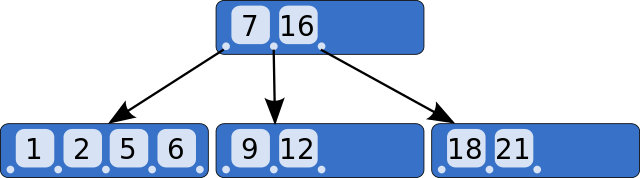
\includegraphics[width=.15\textwidth]{slides_images/b_tree_example}

\end{center}

\end{breakbox}

\begin{breakbox}
\boxtitle{Data Structure for Inverted Index:}

Usually B-trees since they are sorted. Searching for a prefix like 'hyp\%' is now easier since the tree can just be traversed with h->y->p and then collect all children.
\end{breakbox}

\begin{breakbox}
\boxtitle{Blocked Sort-Based Indexing (BSBI):}

Problem of inverted index so far: parse docs one at a time => cannot exploit compression tricks. Solution: Blocked sort-based indexing. Try to keep data as compressed as possible.

\begin{itemize}
	\item External sorting algorithm
	\item Sorting with fewer disk seeks. Basic idea:
		\begin{itemize}
			\item Accumulate postings for each block, sort, write to disk
			\item Then merge the blocks into one long sorted order		
		\end{itemize}
	\item Problem: Keeps dictionary in memory
		\begin{itemize}
			\item Answer: Single-pass in-memory indexing
		\end{itemize}
\end{itemize}
\end{breakbox}


\begin{breakbox}
\boxtitle{Distributed Index:}

\begin{itemize}
	\item Maintain a master machine directing the indexing job -- considered ''safe''
	\item Assign parallel indexing tasks to an idle machine from a pool
	\item Break the input document corpus into splits (corresponding to blocks in BSBI)
	\item on distributed computing clusters which scales (individual machines are fault-prone)
\end{itemize}

Best done with MapReduce.
\end{breakbox}

\begin{breakbox}
\boxtitle{MapReduce:}

A programming (abstraction) model and an associated implementation for processing and generating large data sets.

Phases:
\begin{enumerate}
	\item Map: Each worker node calls Map() for filtering and sorting his own data
	\item Global master node orchestrates that for redundant copies of input data, only one is processed.
	\item Shuffle: Worker nodes redistribute data based on the output keys (produced by the "map()" function), such that all data belonging to one key is located on the same worker node.
	\item Reduce: Worker nodes now process each group of output data, per key, in parallel.
\end{enumerate}

Example for counting words in documents:
\java{java_code/mapreduce_count_words.pseudo}
\end{breakbox}

\begin{breakbox}
\boxtitle{Statistics from Preprocessing}

\begin{itemize}
	\item Stemming and case folding reduce the indexed terms about 17\,\%.
	\item 30 most common words account for 30\,\% of the tokens in written text.
\end{itemize}
\end{breakbox}